\documentclass[a4, titlepage]{article}

\usepackage[czech]{babel}
\usepackage[utf8]{inputenc}
\usepackage[T1]{fontenc}
\usepackage{blindtext}
\usepackage{graphicx}
\graphicspath{ {./img/} }
\usepackage{xcolor}
\usepackage{listings}
\usepackage{hyperref}
\usepackage{subfigure} 
\usepackage{graphicx}

\definecolor{lightgray}{rgb}{0.95, 0.95, 0.95}
\definecolor{purple}{rgb}{0.38,0.18,0.81}
\definecolor{amber}{rgb}{1.0, 0.75, 0.0}
\definecolor{ballblue}{rgb}{0.13, 0.67, 0.8}
\definecolor{cadmiumgreen}{rgb}{0.0, 0.42, 0.24}
\definecolor{cadmiumorange}{rgb}{0.93, 0.53, 0.18}

\hypersetup{
    colorlinks=true,
    linkcolor=ballblue,
    filecolor=magenta,      
    urlcolor=amber,
}

\lstdefinelanguage{JavaScript}{
  keywords={typeof, new, true, false, catch, function, return, null, catch, switch, var, let, cons, if, in, while, do, else, case, break},
  keywordstyle=\color{blue}\bfseries,
  ndkeywords={class, export, boolean, throw, implements, import, this},
  ndkeywordstyle=\color{darkgray}\bfseries,
  morekeywords=[2]{alasql, exec, compile, parse, value},
  keywordstyle=[2]\color{amber}\bfseries,
  morekeywords=[3]{log, for, forEach},
  keywordstyle=[3]\color{purple}\bfseries,
  identifierstyle=\color{black},
  sensitive=false,
  comment=[l]{//},
  morecomment=[s]{/*}{*/},
  commentstyle=\color{red}\ttfamily,
  stringstyle=\color{cadmiumgreen}\ttfamily,
  morestring=[b]',
  morestring=[b]"
}

\lstset{
   backgroundcolor=\color{lightgray},
   extendedchars=true,
   basicstyle=\footnotesize\ttfamily,
   showstringspaces=false,
   showspaces=false,
   tabsize=2,
   breaklines=true,
   showtabs=false,
   captionpos=b
}


\begin{document}

\title{Dokumentace k semestrální práci z předmětu KIV/DBM2}
%\subtitle{AlaSQL}
\author{Bc. Tomáš Vyleta}
\date{21.11.2020}

\maketitle

% Graficka podoba
\begin{figure}
\centering
\subfigure[]{
\includegraphics[width=0.29\textwidth]{javascript_logo}} 
\subfigure[]{
\includegraphics[width=0.39\textwidth]{sql_logo}} 
\subfigure[]{
\includegraphics[width=0.29\textwidth]{alasql_logo}}
\end{figure}

\begin{lstlisting}[language=JavaScript][caption=My Javascript Example]
alasql('ATTACH FILESTORAGE DATABASE test2("./js/file.json");USE test2;',function () {
    console.log(alasql.databases);
});

const myDatabase1 = new alasql.Database();
myDatabase1.exec('CREATE TABLE table1 (number INT)');
myDatabase1.exec('INSERT INTO table1 (number) VALUES (1), (2), (3), (4), (5)');

myDatabase1.exec('SELECT * FROM table1', [],
    function (res) {
        console.log(res);
    }
);

const ceskaMesta = [
    {name: 'Prague', population: 1324277},
    {name: 'Brno', population: 381346},
    {name: 'Ostrava', population: 287968},
    {name: 'Plzen', population: 174842}
];

alasql.databases.myDatabase2.tables.cities.data = ceskaMesta;
vypisVsechnaMesta();
myDatabase2.exec("INSERT INTO cities VALUES ('Rome',2863223),('Paris',2249975),('Berlin',3517424),('Madrid',3041579)");
vypisVsechnaMesta();

const allCities = myDatabase2.exec("SELECT * FROM cities WHERE population < 3500000 ORDER BY population DESC");
console.log(allCities);

myDatabase2.exec('UPDATE cities SET population = population * 1.5 WHERE name LIKE "A%"');
console.log(alasql.databases.myDatabase2);
\end{lstlisting}

\newpage

\tableofcontents
\newpage

\section*{Úvod}
Problémem či zadáním semestrální práce je nalézt a popsat knihovnu pro zpracování množiny souborů ve formátu JSON, které většinou vrací endpointy REST API. Využít ji na úrovni jednoho programu (bez nutnosti vkládání dat do jiných SŘBD pro zpracování objektových souborů). Knihovna by měla být schopna poskytovat funkce obsažené v jazyce SQL jako FROM, GROUP BY, JOIN, atd. Cíle práce jsou: 

\begin{itemize}
	\item Nalezněte existující metody dotazováním se nad množinou JSON souborů.
	\item Popište rozsah nabízených operací ve vybraném jazyce/nástroji.
	\item Analyzujte možnosti jazyka/nástroje v kontrastu s klasickou relační databází resp. SQL.
\end{itemize}


\section{Knihovna AlaSQL}
AlaSQL (čti à la SQL)je \textit{open source} SQL databáze pro JavaScript, operující na straně klienta. Implementuje mnoho funkcí ze čtvrté verze jazyka SQL (SQL:1999) a také některé funkce navíc pro snazší manipulaci s NoSQL a grafovými sítěmi. Také podporuje asynchronní volání pomocí metody promise. Knihovnu lze využít pro webové aplikace, aplikace založené na Node.js nebo v mobilních aplikacích.

Podporuje import/export formátů, jako jsou např. tabulky programu Excel (.xls), CSV - Comma-separated values (.csv), již zmiňovaný JSON - JavaScript Object Notation (.json), TAB - Tab Separated Data File (.tab) a import/export databází IndexedDB, LocalStorage a SQLite.

\begin{figure}[h]
    \centering
    
\includegraphics[width=5cm]{alasql_logo}
    \caption{Logo AlaSQL}
\end{figure}


\subsection{Infobox}
\begin{center}
\begin{tabular}{ ||c|c|| }
\hline
 Jazyk & JavaScript \\
 \hline
 Stabilní verze & v0.6.5 \\
 \hline
 Licence & MIT Licence \\
 \hline
 Vyvíjeno od & 2014 \\
 \hline
 GitHub hvězd & ~5 300 \\
 \hline
 Commity & 2-3/týden \\
 \hline
 Návštěvnost & 2 mil./měsíc  \\
 \hline
\end{tabular}
\end{center}

\subsection{Užitečné odkazy}
\begin{itemize}
	\item WEB: \url{http://alasql.org}
	\item Github: \url{https://github.com/agershun/alasql}
	\item Wiki (Docs): \url{https://github.com/agershun/alasql/wiki}
\end{itemize}

\section{Stack}
Pro práci s knihovnou jsem zvolil \textit{single page} aplikaci, kde všechny dotazy běží na klientovi s podporou JavaScriptu. Aplikace neběží na žádném serveru, tudíž nelze načítat soubory pomocí běžných metod, proto jsou všechna data uložená jako proměnné v JavaScriptu. Pokud ale pracujete s knihovnou v prostředí Node.JS, můžete soubory načítat pomocí \textit{File system} modulu nebo pokud Node.JS nevyužíváte a applikace vám běží na serveru, tak je zde možnost načítat soubory např. pomocí JQuery (asynchronně) nebo pomocí dalších externích knihoven a frameworků. Alasql dokáže načítat soubory asynchronně, ale metody kterými to jde, mají divné ukládání dat viz kapitola \hyperlink{FileLoading}{načítání souborů}.

\section{Instalace}
Knihovna je dostupná v několika JavaScriptových správcích balíčků (package management) kterými jsou npm, Bover a Meteor nebo si ji můžete přímo naklonovat/stáhnout z officiálního GitHub repozitáře. 

Pokud nechcete stahovat knihovnu na fyzické úložiště, nejjednodušší varianta je získat AlaSQL do své aplikace pomocí cloudové služby \href{https://cdnjs.com/libraries/alasql}{cdnjs.com}, která je založena na principu CDN (Content Delivery Network). Stačí tedy do našeho projektu vložit odkaz na tuto knihovnu, např. do hlavičky HTML souboru:

\begin{lstlisting}[language=HTML]
<script src="//cdn.jsdelivr.net/alasql/0.2/alasql.min.js"></script> 
\end{lstlisting}


\section{Použití}
Po úspěšném nainstalovaní/naimportování knihovny jsme schopni ji začít používat. Nyní je několik možností jak s knihovnou pracovat. Chtěl bych zdůraznit, že knihovna vrací vždy pole výsledků nebo JavaScriptový objekt, tabulku pouze v případě, pokud zavoláme metodu tomu určenou.

\subsection{Pomocí funkce}
Všechny dotazy (queries) se vkládají jako atribut metody \textit{alasql(stringWithSQL)} nebo jiné proměnné, pokud si je nazvete, třeba v Node.js. Dotazy lze vykonávat také nad jednotlivou tabulkou nějaké databáze pomocí funkce \textit{exec()} (viz dále).

\subsubsection{NodeJS}
Knihovnu v NodeJS stačí pouze naimportovat, pomocí funkce \textit{require()} o zbytek se vám postará správce balíčků. Použití může vypadat takto:
\begin{lstlisting}[language=JavaScript][caption=My Javascript Example]
var alasql = require('alasql');
alasql('CREATE TABLE one (two INT)');
\end{lstlisting}

\subsection{Nová databáze}
Je tu možnost do proměnné založit novou databázi a nad vytvořenou proměnnou zavolat funkci \textit{exec()} do které vložíme dotaz jako atribut jako v předchozí sekci (funkce \textit{alasql()} je zkrácenou verzí \textit{alasql.exec()}). Můžeme také vkládat více dotazů oddělených ";", kde poté navrácená hodnota bude jako pole výsledků a vy můžete mezi nimi iterovat.

\begin{lstlisting}[language=JavaScript][caption=My Javascript Example]
var mybase = new alasql.Database();
mybase.exec('CREATE TABLE one (two INT)');
\end{lstlisting}

Také k ním můžete přistupovat přes globální objekt \textit{alasql}. Obecně se všechny databáze nacházejí na cestě \textit{alasql.databases.[název databáze]}. To k ním umožňuje jednodušší přístup přes objektovou cestu.

\begin{lstlisting}[language=JavaScript][caption=My Javascript Example]
var mybase = new alasql.Database('mybase');
console.log(alasql.databases.mybase);
\end{lstlisting}

\begin{figure}[h]
    \centering
    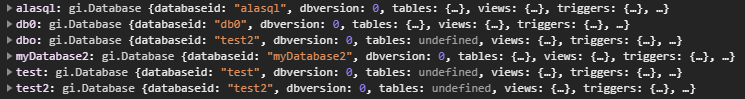
\includegraphics[width=10cm]{databases}
    \caption{Inicializované databáze v objektu \textit{alasql} (příklad)}
\end{figure}

\subsection{Nová tabulka}
Založení nové tabulky je podobné, můžeme ji vytvořit přímo v globálním objektu \textit{alasql} nebo vytvořit uvnitř nějaké databáze. Budu předpokládat, že máme databázi uloženou v proměnné \textit{var mybase}. Pozor, pokud tabulku založíte v globálním objektu alasql, lze k ní přistupovat a vykonávat dotazy přímo přes \textit{alasql()}, pokud ale založíte tabulku v jiné databázi, musíte k ní přistupovat v t= dané databázi (náš případ) pomocí funkce \textit{exec()}. Založení tabulky je pak následující:

\begin{lstlisting}[language=JavaScript][caption=My Javascript Example]
mybase.exec("CREATE TABLE cities (city string, population 
number)");
console.log(alasql.databases.mybase.tables.cities);
console.log(mybase.exec("SELECT * FROM cities"));
\end{lstlisting}

Jak můžete vidět, výpis celé tabulky může být uskutečněn opět pomocí cesty \textit{alasql.databases.[název databáze].tables.[název tabulky]} popř. \textit{alasql.[název tabulky]} nebo jako SQL dotaz nad databází.

\subsubsection{Datové typy}
Datové typy, které jsou dostupné od začátku, tak se dají nalézt v \textit{alasql} objektu pod cestou \textit{alasql.fn.[název nového dat. typu]}. V základu jsou k dispozici tyto datové typy:
\begin{figure}[h]
    \centering
    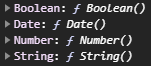
\includegraphics[width=5cm]{fn}
    \caption{Základní datové typy}
\end{figure}

Příklad přidání nového datového typu do objektu databáze:
\begin{lstlisting}[language=JavaScript][caption=My Javascript Example]
// novy datovy typ
alasql.fn.Date = Date;
    alasql('CREATE order (orderno INT, orderdate Date)');
\end{lstlisting}

\subsection{Manipulace dat v tabulce}
Jako jsme zvyklí z SQL, s daty jdou provádět různé úkony, jako je INSERT, UPDATE a DELETE. Syntaxe je stejná jako při založení nové tabulky. Akorát se změní dotaz. Jako příklad mohu uvést:

\begin{lstlisting}[language=JavaScript][caption=My Javascript Example]
mybase.exec("INSERT INTO cities VALUES ('Rome',2863223), 
('Paris',2249975), ('Berlin',3517424),  
('Madrid',3041579)");
\end{lstlisting}

\subsubsection*{INSERT jako JS funkce}
Knihovna umožňuje také vytvářet vlastní metody a jedna z možností je přes funkci \textit{compile()} knihovny, která umožňuje překompilovat příkazy a přidá je do cache dané databáze.

\begin{lstlisting}[language=JavaScript][caption=My Javascript Example]
var insert1 = db.compile('INSERT INTO one (?,?)');
var insert2 = db.compile('INSERT INTO one (:a,:b)');

insert1([1,2]);
insert2({a:3,b:4});
\end{lstlisting}

Funkce \textit{compile()} nejspíše funguje, bohužel pokud jsem zavolal funkci \textit{insert()}, knihovna vyhodila chybu, a tvrdila, že to funkce není. Nenašel jsem nikde řešení.


\subsubsection*{Přidělení dat jako JS objekt}
Určitě vás napadlo, že jako přistupujeme k databázím a tabulkám přes globální objekt, proč by nešlo přistupovat i k datům tabulky nebo je rovnou přiřadit a opravdu to jde. Obecně se všechna data tabulky nacházejí na cestě \textit{alasql.databases.[název databáze].tables.[název tabulky].data}. Příklad objektu na přidělení dat může být následující:

\begin{lstlisting}[language=JavaScript][caption=My Javascript Example]
const ceskaMesta = [
    {name: 'Prague', population: 1324277},
    {name: 'Brno', population: 381346},
    {name: 'Ostrava', population: 287968},
    {name: 'Plzen', population: 174842}
];
alasql.databases.mybase.tables.cities.data = ceskaMesta;
\end{lstlisting}

Je zde ale riziko, přidělená data neprochází přes žádnou funkci, tudíž data vůbec nemusejí odpovídat schématu tabulky, při přidělení dat žádná vyjímka nevyhodí, ale pokud by jsme nad daty zavolali nějaký dotaz, vyskočila by podmínka nebo by data byla \textit{undefiend}. Také pukud vaše tabulka cities již nějaká data obsahuje, toto přiřazení daná data přemaže.

\subsection{Načítání souborů}
\hypertarget{FileLoading}
V dokumentaci je uvedené, že lze zřídit databázi z lokálního souborového systému nebo ze souboru SQLite (místo výroku FILESTORAGE -> SQLITE) a IndexedDB (místo výroku FILESTORAGE -> INDEXEDDB)
\begin{lstlisting}[language=JavaScript][caption=My Javascript Example]
alasql('ATTACH FILESTORAGE DATABASE 
test("./js/file.json")', function () {
    console.log(alasql.databases.test.data);
});
\end{lstlisting}
Vytvoří se databáze s názvem \textit{test} s daty, která jsou v atributu data v dané databázi. Tento atribut pro jinak založené databáze není běžný, jelikož atribut data neobsahují, mají je až obsaženy v tabulkách databáze. Nepřišel jsem na způsob jak nad těmito daty použít dotazy, pouze jak přes adresu proměnné vypsat všechna data nebo dotazovat se pomocí placeholderu s odkazem na data.
Je možné, že podporované databáze mají v souboru založené tabulky a Alasql je sám namapuje, pak lze nad nimi vyvolávat dotazy bez vyhození chyby.

\section{Synchronní/Asynchronní přístup}
Za normálního běhu knihovna vykonává procesy synchronně, ale jdou také volat callbacky nebo asynchronní volání pomocí metody \textit{promise()}. Pokud pracujete se soubory, načítáte je, pak knihovna funguje asynchronně a je doporučeno používat již zmíněnou metodu \textit{promise()}.

\begin{lstlisting}[language=JavaScript][caption=My Javascript Example]
// callback
alasql('SELECT * FROM cities', [],
    function (res) {
        console.log(res);
    }
);

// promise
alasql.promise('SELECT * FROM cities')
    .then(function(res){
    // zpracovani response
    }).catch(function(err){
    // zpracovani chyby
});
\end{lstlisting}

\subsection{HTML}
Knihovna dokáže číst data z HTML tabulky <table>...</table> a výsledek opět vygenerovat do HTML tabulky pomocí CSS selektoru.
\begin{lstlisting}[language=JavaScript][caption=My Javascript Example]
// cteni z tabulky
alasql('SELECT * FROM HTML("#MyTable", {headers:true})');

// zapis do tabulky
alasql('SELECT * INTO HTML("#MyTable", {headers:true}) 
FROM ?',[data]);
\end{lstlisting}


\section{SQL dotazy}
Knihovna je založena, aby co nejvíce připomínala relační databáze s dotazovacím jazykem SQL, podporuje tedy všechny základní výroky SQL jazyka, jako jsou JOIN, GROUP, UNION, ANY, ALL, IN, zanožené dotazy a také správu transakcí. Dále také knihovna podporuje různé agregační metody a dimenzionální funkce, kterými jsou ROLLUP, CUBE a GROUPING SETS. Celý seznam podporovaných funkcí najdete na \url{https://github.com/agershun/alasql/wiki/SQL-99}{SQL-99 features supported by AlaSQL}.

\subsection{Nejlépe funguje s JS}
Tato knihovna je v podstatě SQL databáze v JavaScriptu. Slouží zejména jako podpora zpracování, usnadnění délky kódu, lepší práci s daty nebo jako samostatná client-side databáze - nejlépe však funguje \textbf{SPOLEČNĚ} s JavaScriptem. Knihovna nevrací rovnou tabulky, jak je běžné u relačních databází, ale defaultně vrací data právě jako JSON a další práce s ním je už jako práce s objektem. Sami autoři ve své dokumentaci uvádějí nějaké příklady společně s JavaScriptem a pokud příliš neznáte knihovnu nebo nevíte že nějaké funkce obsahuje, je snazší zpracovat dotaz pomocí JavaScriptu.

\begin{lstlisting}[language=JavaScript][caption=My Javascript Example]
// vypis poctu objektu ve vracenem poli
var db = new alasql.Database();
db.exec('select * from one', function(data) { // callback
   console.log(data.length);						
});

// novy datovy typ
alasql.fn.Date = Date;
    alasql('CREATE order (orderno INT, orderdate Date)');
\end{lstlisting}

\section{Datasety}
\subsection{Rohlík.cz}
K dispozici máme data z webového portálu Rohlik.cz, který se zaměřuje na obchod s potravinami. Data obsahují dva soubory ze dne 2.11.2020, jeden z pohledu obyčejného uživatele (\textit{rohlik2.json}) a druhý z pohledu prémiového uživatele (\textit{rohlik1.json}), hlavní rozdíl mezi těmito dvěma datasety je v ceně za dopravu. Nejvíce nás zajímá atribut \textit{availabilityDays}, který se sestává ze čtyř dalších objektů, popisující dnešek a další následující tři dny. V nich nalezneme atribut \textit{slots}, ve kterém jsou objekty popisující hodiny daný den. V dané hodině nás zajímá atribut \textit{timeSlotCapacityDTO}, který obsahuje konečný atribut \textit{totalFreeCapacityPercent} popisující obsazenost danou hodinu. O úroveň víš je pak atribut \textit{price} značící cenu dovozu.

\subsection{Starcraft}
Druhým datasetem jsou data ze hry Starcraft, máme k dispozici soubory dvou typů. Prvním typem (A) je popis jednotlivých \textbf{tierů}, kterých je dohromady 6, ale k dispozici máme pouze 5. a 6. Dále každý tier obsahuje pole po třech \textbf{divizích (úrovních)} kromě poslední 6. - ta obsahuje pouze jeden. Division má atributy \textit{min\_rating} a \textit{max\_rating} určující rozmezí hráčů. Každý division má pole  obsahuje pole s několika \textbf{laddery}, které již obsahují jednotlivé hráče. Tyto laddery se v průběhu času mění a maximální počet hráčů v jednom ladderu je 100. Laddery popisují soubory typu B, které jsou ve dvou různých datech. Jednotlivé laddery se dají rozeznat podle id a timestampu. V souborech je uložené pole \textit{team} které obsahuje data o jednotlivých hráčích, muhu uvést některé, které budu používat, např. \textit{last\_played\_time\_stamp} - udávající poslední aktivitu hráče v ms, \textit{member[0].legacy\_link.name} - nick hráče s rozeznávacím tagem, \textit{member[0].played\_race\_count.race} - udávající rasu, za kterou hráč hrál, atd.

\section{Důležitá je cesta, ne cíl}
V této sekci popíši všechny dotazy, které jsem pomocí Alasql řešil, jak jsem postupoval a popř. co se mi nepovedlo nebo knihovna nenabízí. 

\subsection{Rohlík.cz}
\subsubsection{Jaké je nejbližší okno s volnou kapacitou?}
Tento dotaz jsem musel řešit s pomocí JavaScriptu, jelikož struktura dat Rohlik.cz v \textit{slots} (rozvozová okénka) jsou atributy a tudíž nelze procházet tento atribut v Alasql jako pole, ale pouze přímými adresami na jednotlivé objekty, pokud chceme projít všechny rozvozová okénka, musíme použít k iteraci JavaScript. V tomto dotazu nám jde o nalezení nejbližšího volného okénka, což je nalezení takové hodnoty, kdy \textit{totalFreeCapacityPercent} je větší než 0: 
\begin{lstlisting}[language=JavaScript][caption=My Javascript Example]
(alasql('SELECT slots FROM ?'
,[rohlikPremium.data.availabilityDays]).forEach(day => {
    for (const [key, value] of Object.entries(day.slots)) {
        const freeCapasity = 
        (alasql('SELECT timeSlotCapacityDTO->totalFreeCapacityPercent 
        AS freeCapacity FROM ?',[value]));
        if (freeCapasity[0].freeCapacity > 0) {
            console.log('Prvni volne okenko dne je: '
             + value[0].since + ' do ' + value[0].till) ;
            break;
        }
    }
}));
\end{lstlisting}
Prvním dotazem vybereme pomocí Alasql atribut \textit{slots}, což je pole (dotaz je zde zbytečný, stačilo pouze přistoupit k poli pomocí JavaScriptu, ale chtěl jsem co nejvíce využívat Alasql). Procházíme každý den. Po té iterujeme každým časovým okénkem pomocí metody for pro iteraci objektů. V každém okénku si necháme pomocí dotazu napsaného v Alasql najít zanořený atribut \textit{totalFreeCapacityPercent} a pomocí podmínky zjistit, jestli je větší jak 0, pokud ne opakujeme a pokud ano, tak necháme časové okénko vypsat a danou iteraci zrušíme pomocí break a iterujeme na další den. Tím se nám vypíší všechny okénka v každém dni:
\begin{figure}[h]
    \centering
    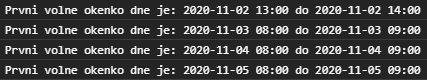
\includegraphics[width=10cm]{R1}
    \caption{Výsledek dotazu Rohlik.cz - 1}
\end{figure}
\newpage

\subsubsection{Kolik volných časových intervalů je k dispozici?}
Tento dotaz je podobný jako první, akorát nechceme pouze najít první volné časové okénko, ale všechny v ten daný den. Tudíž v podmínce nebudeme chtít iteraci přerušit, ale pouze aby pokračovala a pokud tam je volné okénko, tak ho přičíst k nějakému counteru a vypsat pro jednotlivý den, výsledek je: 
\begin{figure}[h]
    \centering
    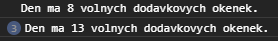
\includegraphics[width=10cm]{R2}
    \caption{Výsledek dotazu Rohlik.cz - 2}
\end{figure}
\newpage

\subsubsection{Jaké je nejbližší nejlevnější okno s volnou kapacitou?}
Tato otázka je podobná jako první, kdy chceme získat první volné okénko, ale k tomu ještě nejlevnější. K řešení musíme použít JSON, který není prémiový, jelikož prémiové členové mají dopravu zdarma. Postup je následující:
\begin{lstlisting}[language=JavaScript][caption=My Javascript Example]
firstFreeDays = [];
(alasql('SELECT slots FROM ?',[rohlikNormal.data.availabilityDays]).forEach(day => {
    for (const [key, value] of Object.entries(day.slots)) {
        const freeCapasity = (alasql('SELECT timeSlotCapacityDTO->totalFreeCapacityPercent AS freeCapacity FROM ?',[value]));
        if (freeCapasity[0].freeCapacity > 0) {
           firstFreeDays.push({od: value[0].since,
                               do: value[0].till,
                               price: value[0].price}) ;
            break;
        }
    }
}));
lowPriceFree = alasql('SELECT * FROM ? WHERE price=(SELECT MIN(price) FROM ?)', [firstFreeDays, firstFreeDays]);
console.log('Prvni nejlevnejsi okno je: od ' + lowPriceFree[0].od + ' do ' + lowPriceFree[0].do + ' s cenou ' + lowPriceFree[0].price + ' Kc.');
\end{lstlisting}
Nejdříve si založíme pole, kam budeme dávat volná okénka pro každý den. Postup je zde stejný jako u první otázky, akorát místo toho aby jsme okénko jen vypsali, uložíme si ho do pole. Po iteraci nad polem zavoláme dotaz, který nám vybere objekt s nejmenší cenou a ten si vypíšeme. Výsledek je takový:
\begin{figure}[h]
    \centering
    
\includegraphics[width=10cm]{R3}
    \caption{Výsledek dotazu Rohlik.cz - 3}
\end{figure}
\newpage

\subsection{Starcraft}
\subsubsection{Kolik hráčů je v jednotlivých divizích/úrovních?}
V této otázce chceme najít celkový počet hráčů na úrovni a v jejích divizích. Nejdříve vybereme všechny divize dané úrovně, poté v každé divizi sečteme počet hráčů ve všech ladderech a nakonec obojí vypíšeme. Vstupním parametrem je tier.
\begin{lstlisting}[language=JavaScript][caption=My Javascript Example]
function sumPlayersFromDivision(tier) {
    let counter = 0;
    for (let i = 0; i < tier.tier.length; i++) {
        memberCount = alasql('SELECT SUM(member_count) AS member_count FROM ?', [tier.tier[i].division]);
        console.log('Tier ' + tier.key.league_id + ' - divize s id ' + tier.tier[i].id + ': ' + memberCount[0].member_count);
        counter  += memberCount[0].member_count;
    }
    console.log('Celkovy pocet hracu v tieru ' + tier.key.league_id + ' je ' + counter);
}
\end{lstlisting}
Zřídíme si counter pro počet hráčů na úrovni. Dále si for cyklem spočítáme/vybereme počet hráčů pomocí funkce SUM() v každé divizi, index zde slouží pro iteraci mezi divizemi. Vypíšeme počet hráčů v divizi a přičteme do counteru. Za tělem for cyklu vypíšeme count, který značí všechny hráče v úrovni. Výsledek je takový: 
\begin{figure}[h]
    \centering
    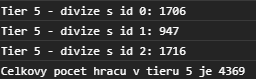
\includegraphics[width=10cm]{S1}
    \caption{Výsledek dotazu Starcraft - 1}
\end{figure}
\newpage

\subsubsection{Jsou konzistentní počty hráčů mezi JSON typ A a B?}
V otázce nás zajímá, zda počet members\_count v JSONu typu A je stejný jako skutečný počet hráču v poli team v JSON typu B. V AlaSQL lze řešit tuto otázku pomocí jednoho volání s dvěma dotazy. 
\begin{lstlisting}[language=JavaScript][caption=My Javascript Example]
function ladderMemberCountConsist(tier, ladderId) {
    count = alasql('SELECT member_count FROM ? WHERE ladder_id= ?;SELECT COUNT(*) AS member_count FROM ?', [tier.tier[0].division, ladderId, ladder230898_1031.team])
    console.log(count);
    console.log('Jsou pocty hracu konzisteni? - ' + (count[0][0].member_count === count[1][0].member_count ? 'ano.' : 'ne.'));
}
\end{lstlisting}
Určím si id ladderu, který mě zajímá a ten naleznu V JSONu typu A pomocí kauzule WHERE a vyberu member\_count. Je zde ale problém, že musím přímo zadat index division, ve kterém se ladder nachází. Tento problém blíže popisuji v kapitole \hyperlink{Error}{Chyby}, jelikož knihovna neumí 2x iterovat. Také se musí přidat ladder (JSON typu B).
V druhém dotazu si spočtu pomocí COUNT() počet záznamů v poli team a vypíši. Pro výpis ještě použiji podmínku if, která výsledek vypíše slovně.
Ladder zde musí být vložen manuálně, jelikož nepracuji se souborovým systémem, řešením by bylo procházet složku s daty a hledat soubor s id daného ladderu. Výsledkem ladderu s id 230898 je:
\begin{figure}[h]
    \centering
    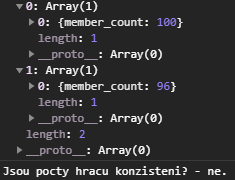
\includegraphics[width=5cm]{S2}
    \caption{Výsledek dotazu Starcraft - 2}
\end{figure}
\newpage

\subsubsection{Seřazení hráčů v rámci jednoho ladderu.}
S touto otázkou si knihovna poradí celkem snadno (bez použití JavaScriptu), pokud chceme seřadit hráče v jednom ladderu a známe id tohoto ladderu. S přiloženými daty si například vezmeme soubor \textit{ladders-eu-230898.json}, což je ladder s \textit{ladder\_id=230898} a pomocí JS můžeme přistupovat k jeho atributům. Všechny hráči daného ladderu jsou uložené v poli \textit{team}. Chceme zobrazit id hráče, k případnému dalšímu dotazování, jméno hráče a rating, což bude seřazená hodnota. Vytvoříme si AlaSQL dotaz:
\begin{lstlisting}[language=JavaScript][caption=My Javascript Example]
function orderPlayersFromLadder(ladderJson) {
    console.log(alasql('SELECT id, rating, member->(0)->character_link->battle_tag AS battle_tag FROM ? ORDER BY rating DESC', [ladderJson.team]));
}
\end{lstlisting}
Vybereme všechny zmíněné atributy. Atribut jména hráče je zanořený, proto musíme volit přístup přes další atributy nebo pole a zobrazíme ho jako battle\_tag, jinak by se celý atribut nazýval podle cesty, které k němu přistupujeme (v tomto případě by se vybraný atribut jmenoval 'member->(0)->character\_link->battle\_tag'). 
Vybraná data můžeme seřadit podle atributu \textit{rating}, pomocí výrazu ORDER BY sestupně nebo vzestupně. Jako výsledek dotazu nad ladderem s ladder\_id=230898 nám dotaz sestrojí následující výsledek:
\begin{figure}[h]
    \centering
    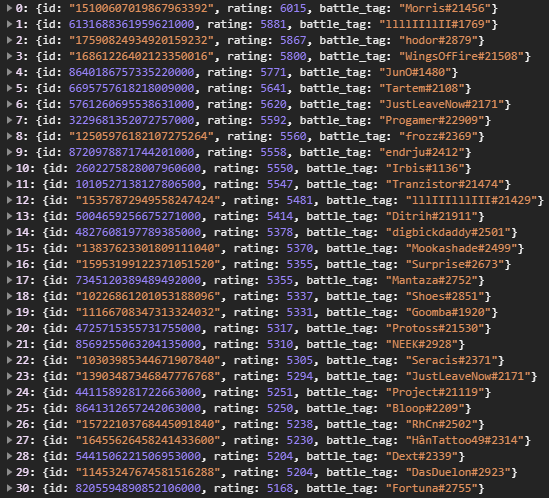
\includegraphics[width=10cm]{S3}
    \caption{Výsledek dotazu Starcraft - 3}
\end{figure}
Jediné na co jsem během tohoto dotazu narazil je, že jsem chtěl, aby si uživatel volil metodu seřazení, jestli ASC nebo DESC přes placeholder pomocí ?, bohužel ale při překladu aplikace padala a vyžadovala již definovanou metodu seřazení vloženou přímo jako string v dotazu.
\newpage

\subsubsection{Kolik hráčů odehrálo v poslední době nějakou hru?}
K tomuto dotazu knihovně opět postačí pouze jeden dotaz, se dvěma vstupními parametry, které nahradíme místo placeholderů a to určitý ladder a konstanta času v ms proti které budeme hráče porovnávat. Alasql dotaz je:
\begin{lstlisting}[language=JavaScript][caption=My Javascript Example]
function lastPlayedFrom(ladderJson, timeFromInMilis) {
    console.log(alasql.exec('SELECT COUNT(*) FROM ? WHERE last_played_time_stamp > ?', [ladderJson.team, timeFromInMilis]));
}
\end{lstlisting}
Chceme zobrazit číslo, tedy počet hráčů, kolik hrálo Starcraft od časové značky. Použijeme agregační funkci COUNT buď s nějakým atributem nebo hvězdičkou, což je v tomto případě jedno. Musíme přidat také klauzuli WHERE a říci, že hledáme hráče, kteří mají \textit{last\_played\_time\_stamp} větší než naše časové razítko. Výsledkem dotazu je:
\begin{figure}[h]
    \centering
    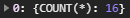
\includegraphics[width=5cm]{S5}
    \caption{Výsledek dotazu Starcraft - 5}
\end{figure} 
\newpage

\subsubsection{Jací hráči jsou v jednom ladderu vícekrát a za jaké rasy?}
Tento dotaz jsem se snažil vyřešit pouze s pomocí Alasql, ale k výsledku jsem se dobral pouze s pomocí JavaScriptu. Vstupním parametrem je jeden ladder.
\begin{lstlisting}[language=JavaScript][caption=My Javascript Example]
function playerMultiRace(ladderJson) {
    result = '';
    temp = alasql('SELECT member->(0)->character_link->battle_tag as name, member->(0)->played_race_count->(0)->race as race FROM ?', [ladderJson.team]);
    alasql('SELECT name FROM ? GROUP BY name HAVING COUNT(*) > 1 ORDER BY name', [temp]).forEach(dupPlayer => {
        result += dupPlayer.name + ': '
        temp.forEach(player => {
            if (dupPlayer.name === player.name) {
                result += player.race + ', ';
            }
        });
        result += '\n';
    });
    console.log(result);
}
\end{lstlisting}
Nejdříve inicializuji prázdný string, který mi bude pomáhat s vypsáním výsledků dotazů. Nejdříve si do proměnné temp zobrazím \textit{battle\_tag} hráčů jako \textit{name} a rasu jako \textit{race} za kterou hráči hráli. V dalším dotazu zobrazím \textit{name} hráče, který se vyskytl v daném ladderu vícekrát. Po té si pomocí JavaScriptu pro každého hráče nechám vypsat jméno a rasy, za které hrál. Výsledek nad ladderem s ladder\_id=230882 vypadá takto:
\begin{figure}[h]
    \centering
    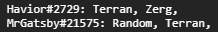
\includegraphics[width=5cm]{S6}
    \caption{Výsledek dotazu Starcraft - 6}
\end{figure} 
\newpage

\subsubsection{Jací hráči přibyli/ubyli v daných ladderech?}
V tomto dotazu chceme porovnat dvě instance stejného ladderu v jiných časových obdobích, tudíž vstupem budou dva zmíněné parametry. Tímto dotazem si Alasql poradí pomocí dvou dotazů nebo jedním zanořeným: 
\begin{lstlisting}[language=JavaScript][caption=My Javascript Example]
function compareLaddersByPlayers(ladderJson1, ladderJson2) {
    union =  (alasql('SELECT member->(0)->character_link->battle_tag as name FROM ? UNION ALL SELECT member->(0)->character_link->battle_tag as name FROM ?', [ladderJson1.team, ladderJson2.team]));
    console.log(alasql('SELECT name FROM ? GROUP BY name HAVING COUNT(*)=1',[union]));
}
\end{lstlisting}
Prvním krokem se sestavení UNION výroku, který vezme z obou instancí battle\_tag hráčů jako \textit{name} a vytvoří z nich pouze jednu tabulku. Nad touto tabulkou zobrazíme pouze ty hráče, kteří se v obou instancích nacházejí pouze jednou. Nevíme ale, jestli daní hráči přibili nebo ubyli. Výsledek dotazů mezi ladderem s ladder\_id=230882 je:
\begin{figure}[h]
    \centering
    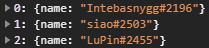
\includegraphics[width=5cm]{S7}
    \caption{Výsledek dotazu Starcraft - 7}
\end{figure} 
\newpage

\subsubsection{Jací hráči vybočují z hranic divizí?}
V dotazu chceme nalézt všechny hráče, kteří patří do jedné divize. Toho docílíme nalezením všech ladderů dané divize. Také potřebujeme získat ELO rozsah dané divize pomocí ukazatelů min\_rating a max\_rating. Až budeme mít všechny hráče z ladderů dané divize, lze jednoduše podle jejich ratingu vyfiltrovat hráče, kteří do rozsahu divize nezapadají. 
\begin{lstlisting}[language=JavaScript][caption=My Javascript Example]
function playersElo(tier, divisionId) {
    division = alasql('SELECT * FROM ? WHERE id= ?', [tier.tier, divisionId]);
    divisionLaddersId = alasql("SELECT ladder_id AS lad_id FROM ?", [division[0].division]);
    // nebo - vybereme divizi a JOINem spojime s ladder ID (SELECT ladder.team FROM ladder INNER JOIN division ON division.ladder=ladder.id)
    // divisionLadders.forEach(ladder => {
    	console.log(alasql('SELECT member->(0)->legacy_link->name AS name, rating FROM ? WHERE rating NOT BETWEEN ? AND ?', [ladder230882_1101.team, division[0].min_rating, division[0].max_rating]));
    // });
}
\end{lstlisting}
Naleznu divizi nebo divize určitého tieru a vyberu min/max každé úrovně, také pole division se všemi laddery kvůli jejich id. Dalším krokem je nalezení všech ladderů z divize. 

V semestrální nepracuji se souborovým systémem a musel bych každý ladder zadat manuálně. Tento krok by šel udělat např. vybrat všechny souborů na základě ladder\_id a načíst je pro další zpracování nebo z jednoho velkého souboru ladderů vybrat ty, které mají stejné id (což by bylo asi časově náročnější). Bohužel v takovém případě nelze udělat JOIN (více tento problém popisuji v kapitole \hyperlink{Error}{Chyby}), důvodem je, že pracujeme nad JSON souborem a ne nad tabulkou - nemáme název tabulky.

Nakonec pro každý ladder vypíšeme name a rating hráčů, kteří nejsou v rozsahu min\_rating a max\_rating divize. Toho docílíme pomocí NOT BETWEEN operátoru. Dané hráče vypíšeme. Výsledek pro jeden ladder je: 
\begin{figure}[h]
    \centering
    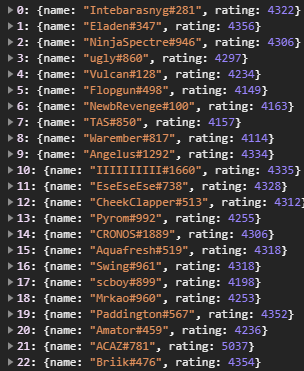
\includegraphics[width=5cm]{S4}
    \caption{Výsledek dotazu Starcraft - 4}
\end{figure} 
\newpage

\subsubsection{Kolik zástupců mají týmy v jednotlivých úrovních?}
Tento dotaz je postupem velice podobný tomu předešlému, musíme nalézt všechny teamy, které jsou v dané diviti a spočítat počet jejich členů. Prvním krokem je výběr divize a nalezení všech ladderů daných divizí v úrovni. Poté získáme všechny clan\_tagy (předpokládám, že funguje jako jednoznačný identifikátor). Po získání všech clan\_tagu necháme je sloučit a sečíst, kolikrát se vyskytují, tím získáme počet hráčů. Jako vstupní parametr nám tedy stačí úroveň. 
\begin{lstlisting}[language=JavaScript][caption=My Javascript Example]
function teamsInTier(tierJson) {
    // vypis vsech ladderu
    let tierLadders = [];
    tierJson.tier.forEach(division => {
        tierLadders.push(alasql("SELECT ladder_id AS lad_id FROM ?", [division.division]));
    });
    // JOIN pres tabulku, kde prvni bude ladder id a druhej sloupec bude nazev ladder souboru
    // SELECT tag, id, COUNT(*) FROM tier INNER JOIN ladders ON league_id=league_id GROUP BY tag
    let teamsMembersCount = [];
    console.log(alasql('SELECT member->(0)->clan_link->clan_tag AS tag, member->(0)->clan_link->id AS id ,COUNT(*) AS members FROM ? GROUP BY member->(0)->clan_link->clan_tag',[ladder230889_1031.team]));
    alasql('SELECT member->(0)->clan_link->clan_tag AS tag, member->(0)->clan_link->id AS id ,COUNT(*) AS members FROM ? GROUP BY member->(0)->clan_link->clan_tag',[ladder230889_1031.team]).forEach(item => {
        teamsMembersCount.push(item);
    });
    alasql('SELECT member->(0)->clan_link->clan_tag AS tag, member->(0)->clan_link->id AS id ,COUNT(*) AS members FROM ? GROUP BY member->(0)->clan_link->clan_tag',[ladder230898_1031.team]).forEach(item => {
        teamsMembersCount.push(item);
    });
    alasql('SELECT member->(0)->clan_link->clan_tag AS tag, member->(0)->clan_link->id AS id ,COUNT(*) AS members FROM ? GROUP BY member->(0)->clan_link->clan_tag',[ladder230882_1031.team]).forEach(item => {
        teamsMembersCount.push(item);
    });
    // nad polem se zgrupujou tymy a secte vyskyt hracu
    console.log(alasql('SELECT tag, SUM(members) FROM ? GROUP BY tag', [teamsMembersCount]));
}
\end{lstlisting}
V prvním kroku vybereme všechny divize úrovně a k nim dané laddery. Tento krok je stejný jako u předchozí otázky, akorát pro všechny divize dané úrovně.
V tomto kroku je také problém jako u minulé otázky, jak vybrat všechny laddery na základě id? Problém a postupy jsem popisoval u předchozí otázky, tudíž to sem nebudu psát znovu. 
Nad každým ladderem vybereme clan\_tag (které jsou v JSON souborech typu B pod každým hráčem) a počet hráčů pomocí metody COUNT(). Navíc s využitím GROUP BY si vybereme všechny týmy jen jednou.
Po té co máme takto zpracované všechny laddery dané úrovně, můžeme je grupovat podle jejich tagu a pomocí agregační metody SUM sečíst výskyt hráčů. V datech se vyskytují hráči, kteří žádný tým nemají, v zadání otázky se na to netážeme, ale pro informaci se může hodit znát. Jako výstup ukíži pouze část výsledků ze 3 ladderů:
\begin{figure}[h]
    \centering
    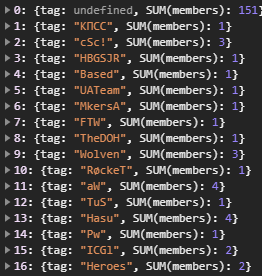
\includegraphics[width=5cm]{S8}
    \caption{Výsledek dotazu Starcraft - 8}
\end{figure} 
\newpage

\subsection{Objevené zajímavé funkce}
\subsubsection*{Placeholder}
Otazník v dotazech je tzv. placeholder. Všechny dotazy, které jsou volány přes Alasql mohou mít v dotazu otazník, který je pak nahrazen hodnotou v poli za výrazem, které obsahuje odkazy na zdroje.

\begin{lstlisting}[language=JavaScript][caption=My Javascript Example]
alasql('SELECT a->b FROM ?',[data]);
\end{lstlisting}

\subsubsection*{Vlastní funkce}
AlaSQL je rozšířitelná a umožňuje nám vytvářet vlastní funkce s použitím JavaScriptu, které pak můžeme zavolat přímo v SQL dotazu. Tato funkcionalita umožňuje široké škálování knihovny a pokud máte s JavaScriptem zacházet, umožňuje vám to vyřešit skoro jakýkoliv problém.

\begin{lstlisting}[language=JavaScript][caption=My Javascript Example]
alasql.aggr.CONCAT = function(v,s) {
    return (s||[]).concat(v);
};

alasql.aggr.LENGTH = function(array) {
	return array.length;
}
\end{lstlisting}

\subsubsection*{Abstract syntax tree}
Umožňuje převádět jazyk SQL na AST (Abstract Syntax Tree), který můžeme programově interpretovat do našeho datového modelu.

\begin{lstlisting}[language=JavaScript][caption=My Javascript Example]
var ast = alasql.parse("SELECT * FROM one");
console.log(ast.toString()); // Vypise puvodni SQL dotaz
\end{lstlisting}
Tato funkce se může použít různě, například pro rychlejší sestavování větších dotazů. Pro představu uvedu strukturu rozloženého objektu:
\begin{figure}[h]
    \centering
    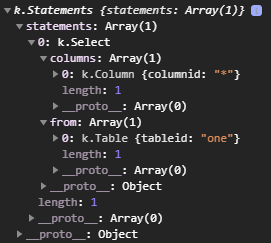
\includegraphics[width=5cm]{astObj}
    \caption{Struktura AST stromu v JavaScriptu}
\end{figure} 

\subsubsection*{pretty(sql)}
Interně, pokud se ve svých dotazech vyznáme, je tato funkce asi zbytečná, ale je dobrá ji mít při vypisování, speciálně dlouhých, dotazů do konzole nebo kamkoliv jinam. Funkce totiž zkrášlí náš stringový dotaz.

\subsubsection*{}
Místo funkcí \textit{alasql()} nebo \textit{exec()} můžete využít také jednu z následujících funkcí:

\begin{lstlisting}[language=JavaScript][caption=My Javascript Example]
alasql.value(sql, params, callback)
alasql.log(sql, params)
\end{lstlisting}

První funkce \textit{value()} vykoná dotaz, ale místo objektu nebo více hodnot vrátí pouze jednu. Druhá funkce \textit{log()} opět vykoná dotaz a rovnou výsledek vypíše do konzole nebo přímo do HTML elementu. Což se velice hodí při debugování.


\section{Chyby}
\subsection{Procházení zanořených objektů}
\hypertarget{Error}
Jako největší chybou nebo nedostatkem jsem se potýkal s problémem, že knihovna nedokáže procházet přes zanořený JSON pomocí jednoho dotazu. Představme si, že máme pole měst a v každém městě je ještě pole okrsků, pokud by jsme chtěli chtěli zjistit/vypsat např. všechny názvy okrsků, šli by jsme na to v AlaSQL nějak takto:
\begin{lstlisting}[language=JavaScript][caption=My Javascript Example]
alasql('SELECT okrsky->name FROM (SELECT okrsky FROM ? WHERE name LIKE 'Praha'), [mesta]);
\end{lstlisting}
Předpokládá se, že knihovna nejdříve vybere všechny okrsky ve městě a pak pro každý okrsek vypíše jméno, bohužel takto jména okrsků nelze získat, pouze to jde nad jedním prvkem v poli, kdy by jsme si museli určit přímo index, který chceme:
\begin{lstlisting}[language=JavaScript][caption=My Javascript Example]
alasql('SELECT okrsky->[0]->name FROM (SELECT okrsky FROM ? WHERE name LIKE 'Praha'), [mesta]);
\end{lstlisting}
Takto dotaz již vrátí výsledky, ale pouze pro první okrsek daného města. V dokumentaci jsem bohužel nenašel žádný způsob, jak by se např. dalo říci, že chci projít celé pole... našel jsem pouze metodu arrayOfArray, ale ta bohužel nefungovala (viz. další kapitola).Proto musíme místo toho použít nějakou iterační metodu JavaScriptu, např. \textit{forEach}. Vybrali by jsme tedy všechny okrsky daného města a nad tímto výsledkem proiterovali dotaz, který by nám vypsal jednotlivé názvy měst.
\begin{lstlisting}[language=JavaScript][caption=My Javascript Example]
alasql('SELECT okrsky FROM ? WHERE name LIKE 'Praha), [mesta]).forEach(okrsek => {
	console.log(alasql('SELECT name FROM ?, [okrsek]);
});
\end{lstlisting}
Tento problém, ale právě řeší JavaScript, který lze bez problému použít, proto možná toto knihovna zbytečně neimplementuje. 

\subsection{Nefunkční}
Další nesnází je nefunkčnost některých metod, které tvůrci uvádějí v dokumentaci, ale pokud je chcete použít, knihovna vyhodí chybu. Mezi takovéto funkce patří například již zmiňovaná \textit{arraayOfArray()}.
Funkce nešli, ani když jsem měl nejnovější verzi knihovny.

\subsection{JOIN}
Funkce JOIN zde existuje a funguje, tudíž bych nechtěl říkat, že je to chyba, ale funguje pouze s vytvořenými tabulkami které máte pojmenované, JSON soubory, které zadáváte přes placeholder bohužel nelze joinovat, jelikož postrádají název. Jako příklad použití JOINu mohu uvést:
\begin{lstlisting}[language=JavaScript][caption=My Javascript Example]
alasql('SELECT city.*, country.* FROM city JOIN country USING countryid');
alasql('SELECT * FROM Cities JOIN Countries USING Country');
\end{lstlisting}

\section{Popis přiložených souborů}
K této dokumentaci také přikládám soubory s příklady a s řešením popsaných otázek. Struktura zip souboru je následující. Po rozbalení je zde jedna složka ..., která je jako root složka projektu v ní se nacházejí složky \textit{dokumetace} - obsahuje dokumentaci ve formátu .pdf, \textit{main} - obsahující HTML a JavaScript soubory a složku \textit{data} - obsahující data poskytnutá k této semestrální práci. pokud půjdeme do složky \textit{main} najdeme zde složky  \textit{data} - která obsahuje některá z poskytnutých dat převedená do JavaScriptu, \textit{js} - obsahující hlavní soubory s kódem a řešení. V main složce jsou také tři HTML soubory, které po otevření v některém z prohlížečů a otevření záložky Console v DevToolu prohlížeče najdete vypsané všechny výsledky dotazů. 

\section{Porovnání s SQL}
Knihovna je primárně navržena aby se s ní co nejvíce pracovalo jako s SQL. Obsahuje všechny základní výroky (SELECT, DISTINC, FIRST, FROM, WHERE, ORDER BY, atd.) agregační funkce (SUM(), AVG(), GROUP BY(), atd.), stringové, numerické, logické a datové funkce (ABS(), UPPER(), YEAR(), ...), JOIN operace (INNER JOIN, LEFT JOIN, OUTER JOIN, ...) a řízení transakcí příkazy (BEGIN, COMMIT a ROLLBACK). 

Jak jsem již zmínil v úvodu, knihovna implementuje mnoho funkcí ze čtvrté verze jazyka SQL (SQL:1999). Přehled, co všechno knihovna podporuje, lze nalézt \href{https://github.com/agershun/alasql}{zde}.  

Pokud si vytvoříte databázi pomocí Alasql, chová se stejně jako SQL databáze, akorát ukládání dat je jiné. Data jsou uložené v JavaScriptovém objektu a máme k nim přístup i bez dotazovacího jazyka přes objektovou cestu. Data je možné ukládat i do Localstorage nebo jiné podporované databáze.

Jak již bylo také zmíněno, knihovna vrací výsledky dotazů jako objekt nebo pole výsledků.

\section{Na závěr}
Celkově se mi s knihovnou dělalo relativně dobře, ALE... pouze při práci společně s JavaScriptem. Dokumentace knihovny pokrývá základy a místy je vidět, že autoři mají připravené odkazy a stránky pro její rozšíření, bohužel je v ní takový celkem zmatek, některé věci jsou na více místech a většina z "live example" nefungují. Odkaz na knihovnu z wiki je ve verzi 0.3.9, což je starší verze, přitom píší, že verze v npm je verzi 0.6.4. Jediné relevantní stránky jsou ty na GitHubu, ostatní stránky v silné většině kopírují obsah a nelze načíst další relevantní zdroj. Bohužel, což mě hodně zklamalo a trošku odradilo jsou funkce, které uvádějí se zajímavými, ne-li potřebnými funkcemi a bohužel, když si je naimplementujete do svého kódu, tak vám to většinou vyhodí exception, že požadovaná funkce zavolaná nad objektem \textit{alasql} není funkcí a nefunguje. 

Na druhou stranu, knihovna nabízí opravdu mnoho zajímavých funkcí a pomocí JavaScriptu jde udělat prakticky cokoliv. Je zde vždy několik cest, jak s knihovnou pracovat, to znamená, že je možné různé problémy řešit různými cestami. Knihovna je velmi populární, podle statistik si ji stáhne cca 13 000 lidí týdně. Leč na knihovně se stále pracuje (soudě podle commitů) a věřím, že autoři opraví stávající problémy a přidají ještě další funkce. Knihovna je opensource, takže kdyby jste potřebovali nějaký projekt na ní založit, můžete. Také pokud vám tam něco chybí, není těžké si udělat vlastní funkci, která toto vykoná. Knihovna se z velké čísti používá jako normální SQL dotazy a uživatel JavaScriptu s ní nebude mít také problémy.

Když jsem vybíral tuto knihovnu, knihovna mě velice zajímala a myslel jsem si, že práce s JSONem nebude problém, bohužel jak jsem začal na semestrální práci pracovat, zjišťoval jsem, že knihovna je spíše založená pro správu relační databáze a úschovu vlastních dat do \textit{LocalStorage} prohlížeče a transformace dat z tabulkových (xls, csv) souborů. Není to přímo určena pro zpracování JSONů, ale základní zpracování umožňuje.

V poslední řadě bych chtěl zmínit špatné chybové hlášky, kdy jsem nevěděl co takový hláška říká. Mnohdy se vám vypíší jen písmenka a pokud nemáte nastudovanou přímo scripty knihovny, tak nevíte, proč to padá. Jako příklad uvádím:
\begin{figure}[h]
    \centering
    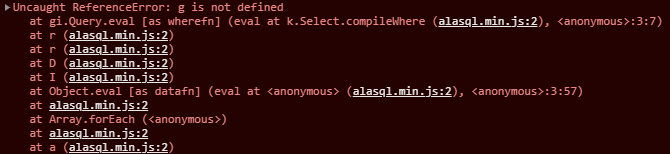
\includegraphics[width=10cm]{error}
    \caption{Příklad vyhozené chybové hlášky}
\end{figure}


\newpage
\begin{thebibliography}{9}
\bibitem{notsoshort}
\textit{Github - AlaSQL} [online]. [cit. 2020-11-16]. Dostupné z: 
\url{https://github.com/agershun/alasql}

\bibitem{notsoshort}
\textit{Github - AlaSQL/Wiki} [online]. [cit. 2020-11-16]. Dostupné z: 
\url{https://github.com/agershun/alasql/wiki}

\bibitem{notsoshort}
\textit{W3C - SQL} [online]. [cit. 2020-11-16]. Dostupné z: 
\url{https://www.w3schools.com/sql/default.asp}

\bibitem{notsoshort}
\textit{cdnjs - alasql} [online]. [cit. 2020-11-16]. Dostupné z: 
\url{https://cdnjs.com/libraries/alasql}

\bibitem{notsoshort}
\textit{DZone - alasql-in-action-the-javascript-sql-database} [online]. [cit. 2020-11-16]. Dostupné z: 
\url{https://dzone.com/articles/alasql-in-action-the-javascript-sql-database}

\bibitem{notsoshort}
\textit{DEV - alasql-a-real-database-for-web-browsers-and-nodejs} [online]. [cit. 2020-11-16]. Dostupné z: 
\url{https://dev.to/jorge_rockr/alasql-a-real-database-for-web-browsers-and-nodejs-24gj}

\end{thebibliography}

\newpage
\listoffigures

\end{document}